%--------------------------------------------------------
% Tema 5. Vectors
%--------------------------------------------------------
\section{Vectors de clonatge}
\label{sec:vectors-de-clonatge}

\subsection{Requisits dels vectors de clonatge}
\label{sec:requ-dels-vect}

Han de tenir les següents característiques:
\begin{itemize}
\item Penetrar i mantenir-se a la cèl·lula hoste
\item Replicar-se a la cèl·lula hoste: Ha de tenir un origen de
  replicació adequat per la cèl·lula hoste. El vector es pot integrar
  de forma episomal o mantenir-se independent com a forma plasmídica.
\item Marcador genètic per la seva selecció: Els més utilitzats són
  els gens de resistència a antibiòtics. Després es suplementa el medi
  de creixement amb aquest antibiòtic per seleccionar els bacteris que
  han integrat el plàsmid.
\end{itemize}

La majoria de vectors són d'origen natural.

Hi ha els següents tipus de vectors:
\begin{itemize}
\item Plàsmids
\item Genoma de bacteriòfags (incloent els còsmids)
\item Vectors per llevats
\item Vectors per eucariotes superiors
\end{itemize}

La capacitat de càrrega d'un plàsmid (mida de l'insert) és de 3-4 kb.

Una característica important són els \textbf{grups d'incompatibilitat} dels
plàsmids, són plàsmids que tenen el mateix origen de replicació i que
no poden coexistir en una cèl·lula hoste. Si es volen clonar 2 gens es
pot fer en tàndem en 1 mateix plàsmid o en 2 plàsmids amb origens de
replicació diferents.

Hi poden haver diferents còpies del plàsmid en una mateixa cèl·lula:
hi ha plàsmids \textit{high copy} o \textit{low copy}.

\subsection{Manipulació de plàsmids}
\label{sec:manip-de-plasm}

\subsubsection{Plàsmid pBR322}
\label{sec:constr-del-plasm}

Es va partir del ColE1 i es va extraure l'origen de replicació. Es va
digerir i es va introduir un cassette de resistència a ampicil·lina
de R1. Es va introduir un altre cassette de resistència a
antibiòtics. La idea d'introduir 2 cassettes de resistència és
diferenciar els clons recombinants si l'insert trunca 1 dels 2
cassettes.

\begin{figure}[H]
  \centering
  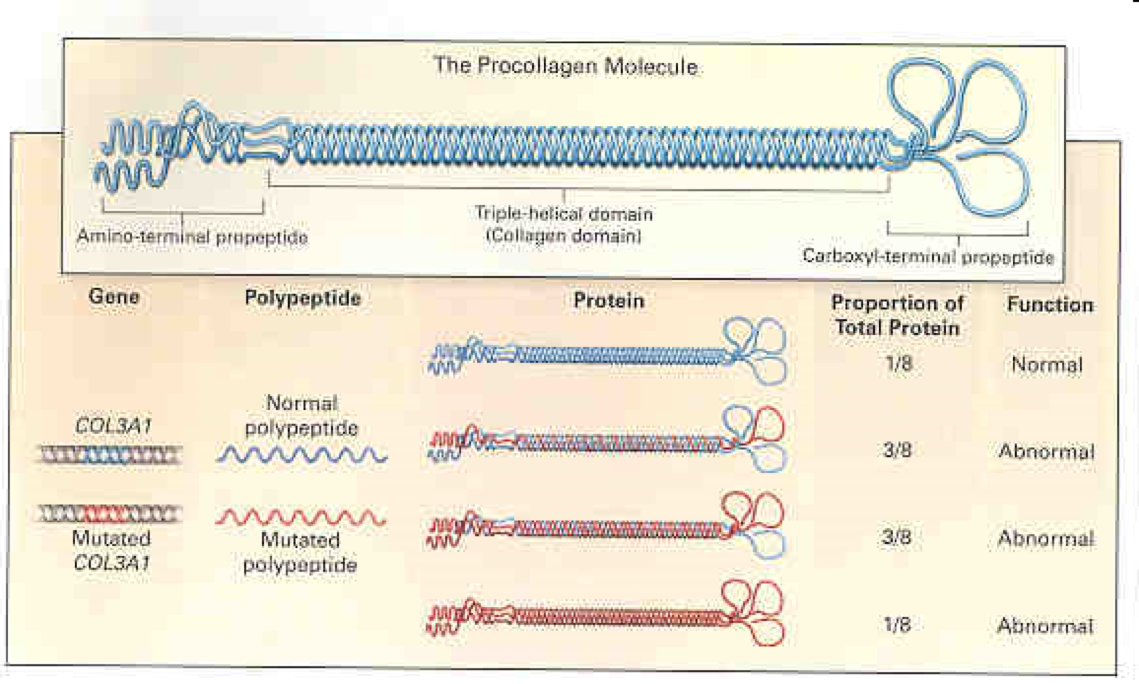
\includegraphics[width=0.75\textwidth]{fig24}
  \caption{Obtenció original de pBR322}
  \label{fig:fig24}
\end{figure}

Es clona un gen dins el vector usant BamHI. Això provoca que es
trenqui el cassette de resistència a tetraciclina.

\begin{figure}[H]
  \centering
  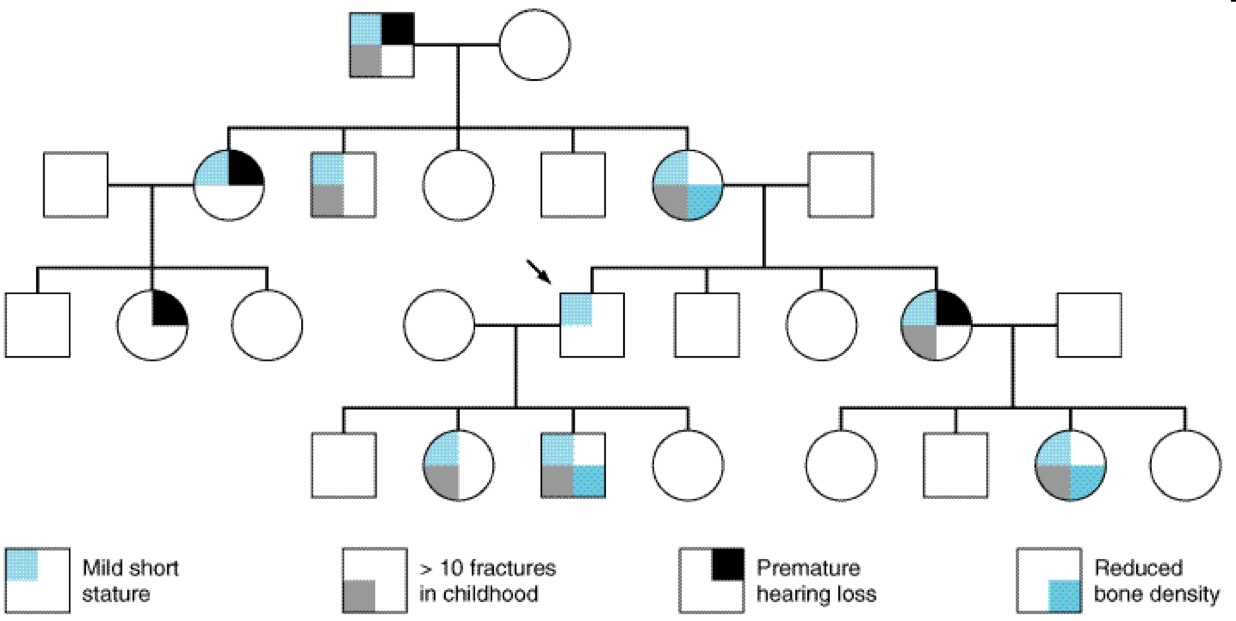
\includegraphics[width=0.75\textwidth]{fig25}
  \caption{Clonatge d'un gen a pBR322}
  \label{fig:fig25}
\end{figure}

La selecció es fa en 2 passos: En 1 placa amb ampicilina i altra amb
tetraciclina i es plaquegen les colònies en la mateixa
posició. S'incuben i es mira quines colònies han crescut. Si la
colònia ha crescut en les 2 plaques, es descarta ja que només hi ha el
plàsmid nu. S'agafen les colònies que només en crescut en
ampicil·lina.

\begin{figure}[H]
  \centering
  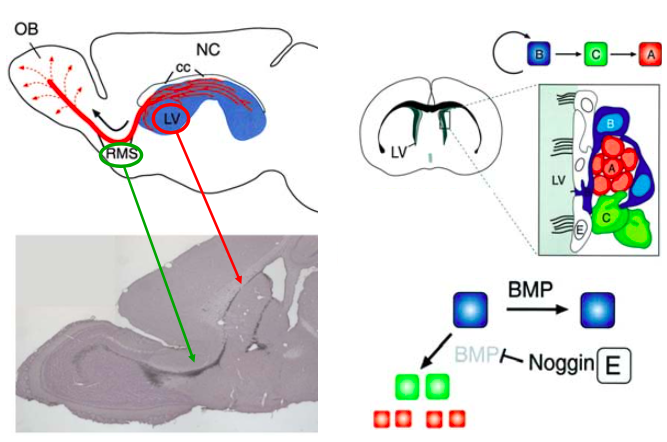
\includegraphics[width=0.75\textwidth]{fig26}
  \caption{Selecció dels transformants per pBR322}
  \label{fig:fig26}
\end{figure}

\subsubsection{Plàsmid pUC8}
\label{sec:plasmid-puc8}
Encara que la inactivació insercional d'un gen de resistència a
antibiòtics doni una bona manera d'identificar els recombinants, el
mètode necessita 2 identificacions (pels transformants i els
recombinants). El pUC8 porta un gen de resistència a ampicil·lina i el
gen lacZ', que codifica per una part de la $\beta$-galactosidasa. El
clonatge amb pUC8 implica la inactivació insercional del gen lacZ', i
els recombinants s'identifiquen per la incapacitat de produir
$\beta$-galactosidasa.

\begin{figure}[H]
  \centering
  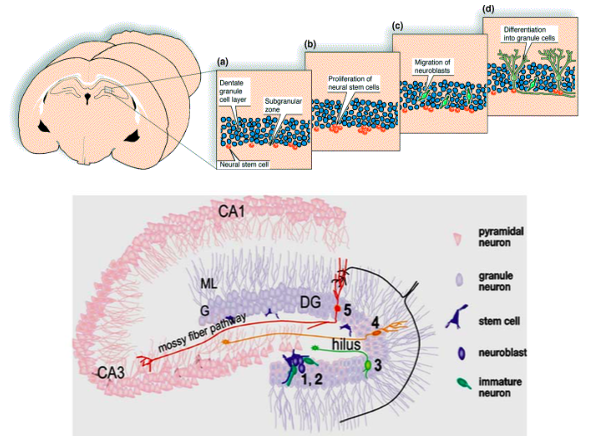
\includegraphics[width=0.75\textwidth]{fig27}
  \caption{Clonatge amb pUC8}
  \label{fig:fig27}
\end{figure}

Algunes soques d'\textit{E. coli} tenen un gen lacZ modificat, que
falta la part codificada per lacZ' de la
$\beta$-galactosidasa. Aquests mutants només poden sintetitzar l'enzim
si duen el pUC8.

Les cèl·lules que tenen pUC8 són resistents a l'ampicil·lina i són
capaces de sintetitzar la $\beta$-galactosidasa; els recombinants són
resistents a ampicil·lina però incapaços de sintetitzar
$\beta$-galactosidasa.

Això implica afegir a la placa d'agar X-Gal, que quan s'hidrolitza
produeix una coloració blava. A més, s'afegeix IPTG (inductor de
l'enzim) i ampicil·lina:
\begin{itemize}
\item Si la colònia és de color blau: la galactosidasa hidrolitza
  X-Gal i per tant no és recombinant (és a dir l'insert no s'ha lligat
  a la zona polilinker de lacZ').

\item Si la colònia és de color blanc: la galactosidasa no és
  funcional i per tant l'insert s'ha lligat a la zona polilinker.
\end{itemize}

El pUC8 permet seleccionar transformants i recombinants en 1 sol pas.

pLac és un promotor induïble per IPTG. Així a la placa de cultiu s'ha
de posar l'antibiòtic (ampicil·lina), X-Gal i IPTG.

\subsubsection{Fagèmids}
\label{sec:fagemids}

Són plàsmids que tenen seqüències de fags. pEMBL8 té un gen de
resistència a ampicil·lina, lacZ' i seqüències M13, que permetin
induir còpies de DNA senzill i puguin ser empaquetades en un fag.

\subsection{Vectors d'expressió}
\label{sec:vectors-dexpressio}

Els vectors d'expressió tenen un promotor fort, una caixa
Shine-Dalgarno i la seqüència codificant. Molts vectors tenen
seqüències terminadores.

Els promotors dels vectors d'expressió poden ser:
\begin{itemize}
\item Induïbles: A nivell basal no hi ha expressió. Quan s'introdueix
  un efector positiu, s'activa l'expressió del gen. Exemple de l'operó
  Lac induïble per IPTG.

\item Repressibles: A nivell basal hi ha expressió. La introducció
  d'un efector provoca el silenciament de l'expressió. Exemple de
  l'operó Trp reprimible per triptòfan.
\end{itemize}

Quan s'expressen gens heterològament hi poden haver problemes amb la
traducció (col·locació correcta dels aminoàcids en funció dels
codons), plegament correcte... Per això es fan proteïnes de fusió. El
que es fa és clonar l'insert enganxat a un gen bacterià sense alterar
la pauta de lectura.

\subsection{Vectors derivats del fag $\lambda$}
\label{sec:vectors-derivats-del}

El genoma del fag $\lambda$ té una regió que no és essencial pel seu
cicle vital. El genoma de $\lambda$ pot circularitzar perquè té unes
regions als extrems de cadena senzilla que són complementaris. Aquests
extrems s'anomenen \textit{cos}. El genoma de $\lambda$ de forma
episòmica es replica com a cercle rodant de forma concatenada. Un
enzim de $\lambda$ reconeix les seqüències cos i les talla. El fag $\lambda$
reconeix els extrems cos i els empaqueta. Els fragments que es poden
clonar en aquesta regió no essencial han de ser d'unes 3 kb.

Hi ha 2 problemes bàsics per clonar amb el fag $\lambda$:
\begin{enumerate}
\item Els inserts que accepta $\lambda$ han de ser iguals o inferiors
  a 3 kb. Si la mida total del vector és superior a 52kb, no es pot
  empaquetar a l'estructura de $\lambda$ i no es formen partícules
  infectives.

\item El genoma de $\lambda$ té múltiples doanes de restricció, per
  tant no es poden usar endonucleases per obrir el vector i clonar un insert.
\end{enumerate}

Hi ha 2 vectors derivats de $\lambda$:
\begin{itemize}
\item \textbf{Vectors d'inserció:} S'ha eliminat la zona no essencial i s'ha
  introduït una diana de restricció. 

\begin{figure}[H]
  \centering
  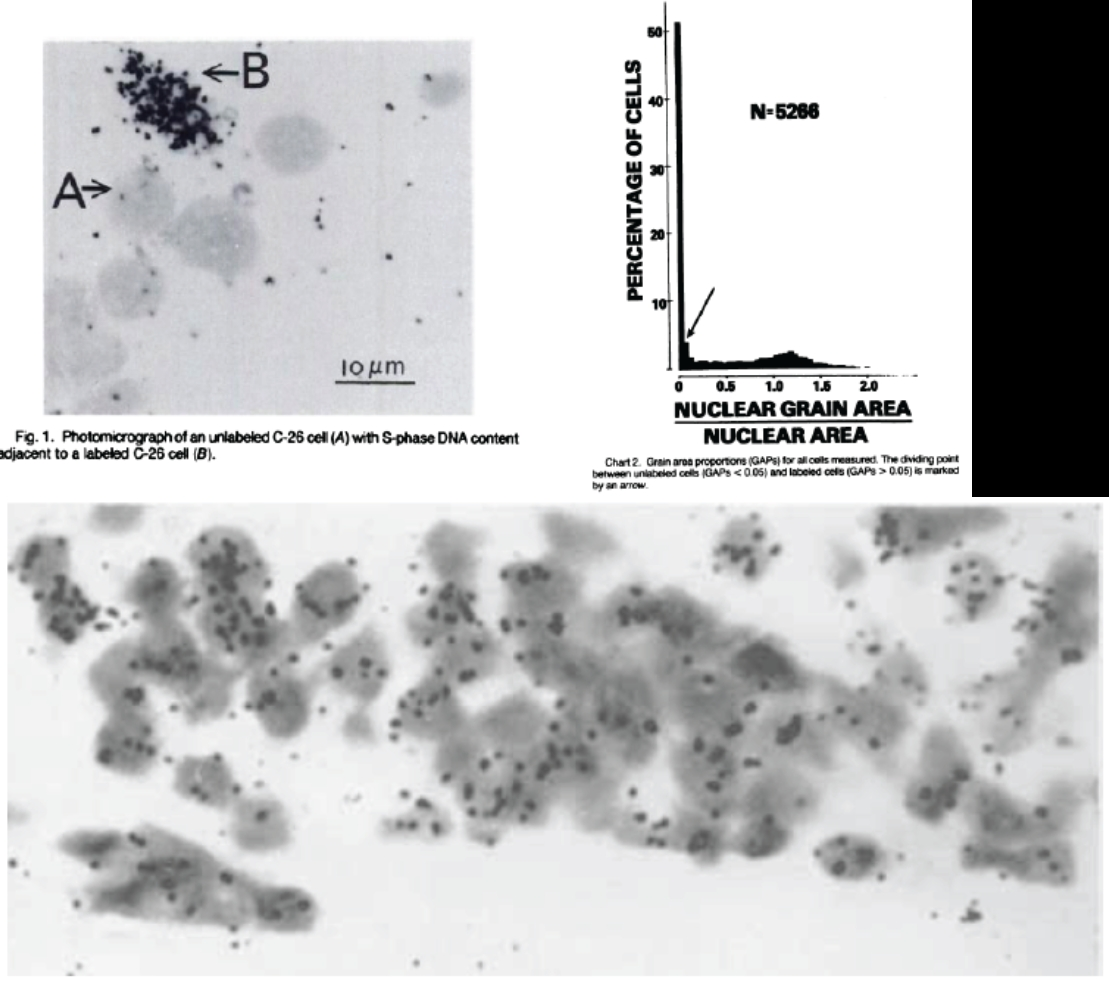
\includegraphics[width=0.75\textwidth]{fig28}
  \caption{Construcció d'un vector d'inserció}
  \label{fig:fig28}
\end{figure}

  \begin{itemize}
  \item $\lambda$gt10 porta una diana
  EcoRI al gen cI (controla el cicle lisogènic). Els fags que tinguin
  un insert en cI tindran cicle lític i els que no seguiran un cicle
  lisogènic. Les calbes transparents suposen que $\lambda$ segueix un
  cicle lític i per tant són recombinants; llavors es fa un raspat de
  les calbes i es recupera el fag recombinant. Si hi ha calbes tèrboles,
  vol dir que no hi ha fag recombinant.

  \item $\lambda$zapIII porta el gen lacZ' amb una diana a
    l'interior. S'introdueix en un bacteri que porti l'altre lacZ amb
    X-gal i IPTG. Si les colònies són clares vol dir que el fag és
    recombinant, si són blaves vol dir que el fag no és recombinant.
  \end{itemize}

\begin{figure}[H]
  \centering
  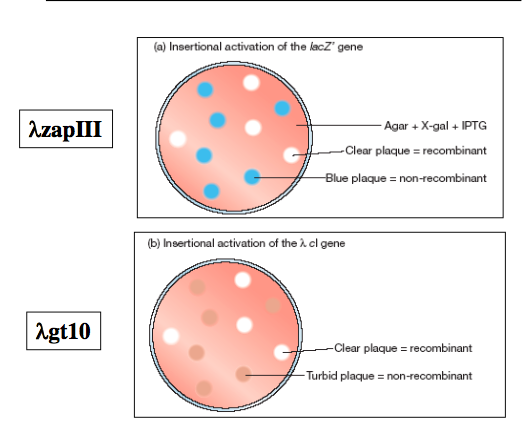
\includegraphics[width=0.75\textwidth]{fig29}
  \caption{Selecció de transformants amb vectors d'inserció de $\lambda$}
  \label{fig:fig29}
\end{figure}

\item \textbf{Vectors de substitució:} Té 2 dianes de restricció que
  es poden usar per clonar. Aquestes dianes flanquejen un segment de
  DNA que és substituït pel DNA a clonar. Sovint el fragment que es
  substitueix porta una diana de restricció addicional que es pot usar
  per tallar-la en fragments petits i evitar la pròpia
  reinserció. Poden carregar fragments de DNA més grans que els
  vectors d'inserció. Els vectors no recombinants són massa petits per
  empaquetar-los en partícules infectives de $\lambda$.

\begin{figure}[H]
  \centering
  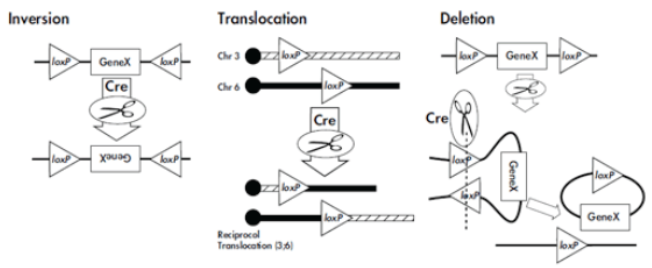
\includegraphics[width=0.75\textwidth]{fig30}
  \caption{Clonatge amb vectors de substitució de $\lambda$}
  \label{fig:fig30}
\end{figure}

El vector $\lambda$EMBL4 pot carregar fins a 20 kb de DNA reemplaçant
un fragment flanquejat per EcoRI, BamHI, SalI. Qualsevol d'aquests
enzims es pot usar per eliminar el DNA reemplaçable. La selecció és:
\begin{itemize}
\item Mida
\item Fenotip Spi: El fag $\lambda$ normalment no pot infectar
  \textit{E. coli} que ja tinguin un altre fag integrat. Llavors es
  diu que $\lambda$ és Spi+. Hi ha cèl·lules mutants que porten P2
  però es poden infectar per un altre fag, pel que els recombinants
  Spi- formen plaques i la resta no.
\end{itemize}
\end{itemize}

Un experiment de clonatge amb $\lambda$ es pot fer com si fos un
plàsmid normal. El DNA de $\lambda$ es digereix, s'afegeix el nou DNA,
es lliga la barreja, i les molècules resultants es transfecten a un
cultiu d'\textit{E. coli}. Aquest tipus d'experiment requereix que el
vector estigui en forma circular.

A vegades, una simple transfecció no és particularment eficient. Es
pot obtenir un gran nombre de recombinants amb algunes
modificacions. El primer és usant el vector linearitzat. Quan el
vector lineal es difgereix, s'alliberen els braços dret i esquerre com
a fragments separats. La molècula recombinant es pot obtenir barrejant
el DNA a clonar amb els braços del vector. La lligació resulta en
reorganitzacions moleculars, incloent la repetició de catetanes. Si
l'insert és de mida correcta, els llocs cos que separen aquestes
estructures estaran a la distància correcta per ser empaquetades
\textit{in vitro}. Després, es pot infectar un cultiu bacterià amb
aquests fags.

\begin{figure}[H]
  \centering
  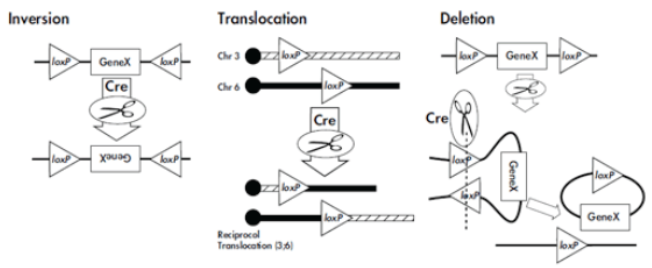
\includegraphics[width=0.75\textwidth]{fig30}
  \label{fig:fig31}
\end{figure}

\subsubsection{Còsmids}
\label{sec:cosmids}
Els còsmids són híbrids entre una molècula de fag i un plàsmid
bacterià, i es basen en l'ús dels llocs cos. L'empaquetament en
partícules fàgiques funciona amb qualsevol molècula de DNA amb llocs
cos separats per 37-52 kb de DNA.

\begin{figure}[H]
  \centering
  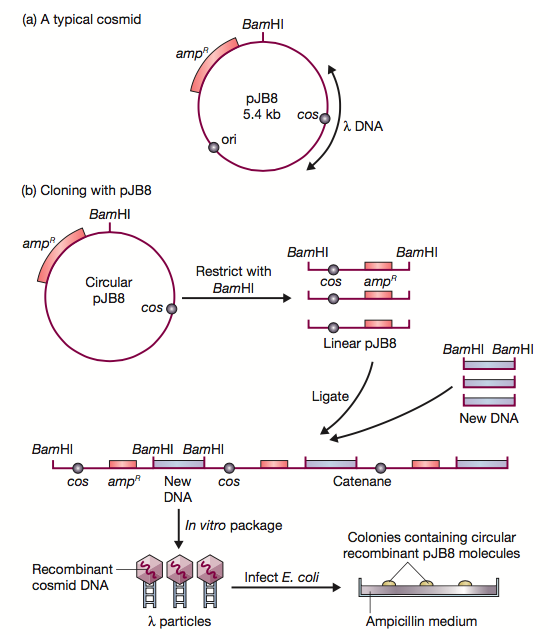
\includegraphics[width=0.75\textwidth]{fig32}
  \label{fig:fig32}
\end{figure}

Un còsmid és un plàsmid amb un lloc cos. També necessita un marcador
de selecció, com el gen de resistència a l'ampicil·lina, i un origen
de replicació adequat. Els còsmids no produeixen calbes de lisi. 

Providing the inserted DNA is the right size, in vitro
packaging cleaves the cos sites and places the recombinant cosmids in
mature phage particles. These lambda phage are then used to infect an
E. coli culture, though of course plaques are not formed. Instead,
infected cells are plated onto a selective medium and
antibiotic-resistant colonies are grown. All colonies are recom-
binants, as non-recombinant linear cosmids are too small to be
packaged into lambda heads.

Un experiment de clonatge amb còsmids, primer s'ha d'obrir el còsmid
amb un únic lloc de restricció i lligar els fragments de DNA. Aquests
fragments són produïts per una digestió parcial amb una endonucleasa,
ja que la digestió total resulta en fragments que són massa petits per
ser clonats a un còsmid. La lligació es fa per permetre la formació de
les catenanes. Proporcionant l'insert de DNA de mida adequada,
l'encapsidació \textit{in vitro} s'escindeix als llocs cos i col·loca
els còsmids recombinants en partícules de fag madures. Aquests fags
$\lambda$ s'utilitzen llavors per infectar un cultiu
d'\textit{E. coli}, encara que no es formin calbes de lisi. En lloc
d'això, les cèl·lules infectades es col·loquen en plaques sobre un
medi selectiu i les colònies resistents als antibiòtics creixen. Totes les colònies
són recombinants, com còsmids lineals no recombinants són massa petits
per a ser empaquetat en partícules $\lambda$.